% This file was created by tikzplotlib v0.9.2.
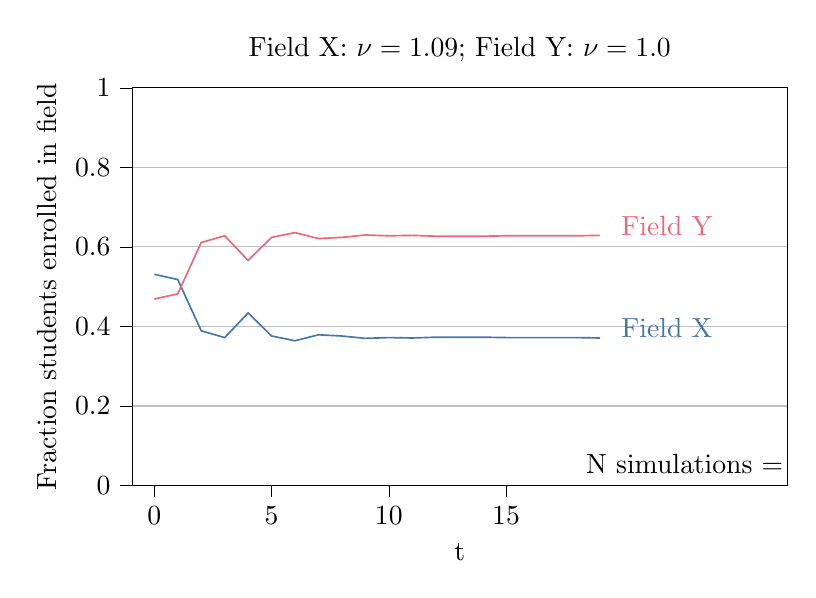
\begin{tikzpicture}

\definecolor{color0}{rgb}{0.266666666666667,0.466666666666667,0.666666666666667}
\definecolor{color1}{rgb}{0.933333333333333,0.4,0.466666666666667}

\begin{axis}[
height=6.6314113761540705cm,
tick align=outside,
tick pos=left,
title={Field X: \(\displaystyle \nu=1.09\); Field Y: \(\displaystyle \nu=1.0\)},
width=9.904475999999999cm,
x grid style={white!69.0196078431373!black},
xlabel={t},
xmin=-0.95, xmax=27,
xtick style={color=black},
xtick={0,5,10,15},
xticklabels={\(\displaystyle 0\),\(\displaystyle 5\),\(\displaystyle 10\),\(\displaystyle 15\)},
ylabel={Fraction students enrolled in field},
ymajorgrids,
ymin=0, ymax=1,
ytick style={color=black},
ytick={0,0.2,0.4,0.6,0.8,1},
yticklabels={\(\displaystyle 0\),\(\displaystyle 0.2\),\(\displaystyle 0.4\),\(\displaystyle 0.6\),\(\displaystyle 0.8\),\(\displaystyle 1\)}
]
\addplot [semithick, color0]
table {%
0 0.531000018119812
1 0.51800000667572
2 0.388999938964844
3 0.371999979019165
4 0.434000015258789
5 0.375999927520752
6 0.363999962806702
7 0.378999948501587
8 0.375999927520752
9 0.370000004768372
10 0.371999979019165
11 0.371000051498413
12 0.373000025749207
14 0.373000025749207
15 0.371999979019165
18 0.371999979019165
19 0.371000051498413
};
\addplot [semithick, color1]
table {%
0 0.468999981880188
1 0.48199999332428
2 0.611000061035156
3 0.628000020980835
4 0.565999984741211
5 0.624000072479248
6 0.635999917984009
7 0.621000051498413
8 0.624000072479248
9 0.629999995231628
10 0.628000020980835
11 0.628999948501587
12 0.626999974250793
14 0.626999974250793
15 0.628000020980835
18 0.628000020980835
19 0.628999948501587
};
\draw (axis cs:19.5,0.371) node[
  anchor=base west,
  text=color0,
  rotate=0.0
]{Field X};
\draw (axis cs:19.5,0.629) node[
  anchor=base west,
  text=color1,
  rotate=0.0
]{Field Y};
\draw (axis cs:18,0.03) node[
  anchor=base west,
  text=black,
  rotate=0.0
]{N simulations = 1000};
\end{axis}

\end{tikzpicture}
